\section{Clustering}
This section explains the various cluster algorithms used in the research.
Subsequently, we will explain and indicate how the hyperparameters are handled in the research for each algorithm.
\subsection{Types of cluster algorithms}
Multiple cluster types can be utilized for clustering data \citep{xu_comprehensive_2015}.
For this study, we selected the types that use some form of distance for clustering.
We explain each cluster type with corresponding cluster algorithms.
\subsubsection{Partition based clustering}
With this type, the data is partitioned and allocated into a fixed amount of clusters.
A well-known and popular cluster algorithm is K-means.
Based on Loyd et al.'s original method, this algorithm randomly selects $k$ points as cluster centroids \citep{1056489}.
Iteratively each data point is assigned to its nearest centroid.
It keeps proceeding until the distance between the cluster centroids is optimal.
%The algorithm can also be used in a distributed manner.
%Instead of calculating the centroids locally, each party receives the centroids and calculates their nearest centroids [Xia et al., 2020].
Although K-means serves its purpose well, it requires pre-defining the number of clusters and is sensitive to outliers \citep{keller_balancing_2021}.
Therefore, a parameterless alternative to K-means is \gls{ap} \citep{frey_clustering_2007}.

\gls{ap} is an algorithm that clusters data points by iteratively passing messages between them.
Each point sends and receives messages about the attractiveness of other points as cluster centers (exemplars) and the suitability of itself as a center \citep{keller_balancing_2021}.

\subsubsection{Density based clustering}
The data points are partitioned for this clustering type based on nearest neighbors \citep{fahad_survey_2014}.
A region with a high data density is considered a cluster \citep{xu_comprehensive_2015}.
A popular density-based cluster algorithm is \gls{dbscan}.
The method was introduced by Ester et al. and worked by drawing a radius ($radius(\epsilon)$, not to be confused with the privacy budget $\epsilon$) around data points \citep{ester_density-based_nodate}.
It then groups all points within this radius as clusters.
The main advantage is its ability to find arbitrarily shaped clusters and detect outliers \citep{liu_privacy_2012}.

Another density-based algorithm is \gls{optics}, an extension of \gls{dbscan}.
This algorithm attempts different $radius(\epsilon)$ values to achieve the best result \citep{ankerst_optics_nodate}.
Instead of directly assigning data points to clusters, specific distance calculations are stored in a list.
For each data point, it tracks two values: core distance and reachability distance.
These values represent the shortest distance to make a data point, $p$, a core point, and the shortest distance from $p$ to another core point, $p'$, respectively.
A specific ordering is maintained to ensure that clusters with higher density values are processed first.
Based on this ordering, the \gls{dbscan} algorithm is constructed hierarchically \citep{schubert_dbscan_2017}.


\subsubsection{Hierarchical clustering}
The name originates from the way hierarchical clustering works.
A hierarchy of clusters is generated and merged according to the closeness of data points \citep{meng_private_2021}.
One of the best known Hierarchical cluster algorithms is \gls{birch}.
This algorithm works by constructing a tree with nodes (so-called clustering feature) \citep{zhang_birch_1996}.
The algorithm does this iteratively until a cluster becomes too large or diverse.
The algorithm will split again into similar clusters until all data is processed \citep{zhang_birch_1996}.

\subsubsection{Research direction}
Based on the different types of clustering algorithms, we have chosen to apply both partition-based clustering algorithms in this research.
K-Means, widely used in the literature, will be utilized alongside the parameterless alternative, \gls{ap}.

For density-based clustering, we will solely focus on OPTICS in this study.
The parameter $radius (\epsilon)$ in \gls{dbscan} is influenced by the data shape, which is further affected by our privacy mechanism.
However, as \gls{optics} automatically determines the $radius(\epsilon)$, the impact of this parameter is less significant, enabling us to emphasize the evaluation of the privacy mechanism itself.

As for hierarchical clustering, we have decided to exclude it from the initial scope of the research.
This type of clustering presents substantial differences in its approach compared to the other clustering algorithms.
Consequently, we will concentrate on partition-based and density-based clustering methods for the current investigation, ensuring a more cohesive and manageable research scope.

%Because the \gls{dbscan}'s $epsilon'$ algorithm is sensitive to the shape $epsilon'$ value, we utilize \gls{optics} for this research instead of \gls{dbscan}.

%Another density-based cluster method is Density Peak Clustering (DPC). 
%The algorithm calculates the local density of each data point and identifies density peaks for points with the highest density [Rodriguez and Laio, 2014].

\subsection{Parameter selection}
A list of important hyperparameters that can influence the results is provided for each clustering algorithm.
Subsequently, we briefly discuss the methods for determining these hyperparameters for the algorithms. \newline
We use the same distance function for all algorithms to have all the algorithms in the same setting.
This function will be Euclidean distance, as used for \gls{gi}.
\subsubsection{K-Means} \label{theory:kmeans}
The most crucial parameter of the K-Means algorithm is the value of $k$.
This value determines the number of clusters to consider and influences the results by a lot \citep{ahmed_k-means_2020}.
%These methods require a manual way of selecting the best $k$ by visual inspection of a plot.
The first method is called an "elbow" plot \citep{kodinariya_review_2013}.
This method finds the best $k$ by applying the K-Means algorithm multiple times and estimating the best $k$.
\begin{figure}[H]
  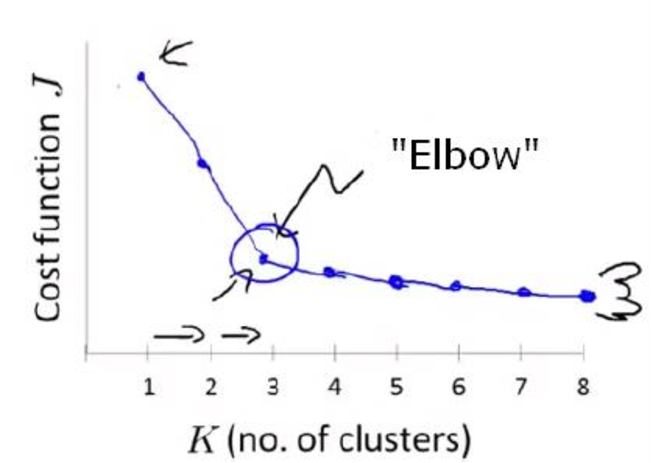
\includegraphics{TheorethicalFramework/dentification-of-Elbow-point.png}
  \caption{Illustration of determining $k$ using the "elbow" method \citep{kodinariya_review_2013}}
\end{figure}
In this situation, a Silhouette plot can be used to determine the $k$.
This method uses the Silhouette coefficient for each cluster \citep{saputra_effect_2020}.
Because this metric measures the separation and cohesion of the cluster, it can be used to choose an optimal amount of clusters \citep{saputra_effect_2020}.
%The plot can then be made by plotting the silhouette coefficient on the y-axis and $k$ on the x-axis .
By visualizing the silhouette scores, the K with the highest coefficient has the best-separated clusters. \newline
Another method is the Gap statistic method \citep{yuan_research_2019}.
It compares the total within-cluster variation for different values of k with their expected values under a null reference distribution of the data \citep{tibshirani_estimating_2001}.
A practical appliance of this method uses a line plot for comparing the $k$-value and gap value \citep{yuan_research_2019}.
Based on the line's visual change, someone can select the best $k$ (the "elbow").

In summary, no fixed method exists to choose a good $k$ for K-Means.
The elbow method is standard in the existing literature and is very popular due to its simplicity.
However, one disadvantage is that it can be challenging to determine the "elbow" point, as it is not always present \citep{kodinariya_review_2013}.
In that case, the silhouette or gap statistic method is a good alternative, where the silhouette score is the simpler method.
\subsubsection{Affinity Propagation} \label{theory:clustering-ap}
%\gls{ap} is an algorithm that clusters data points by iteratively passing messages between them.
%Each point sends and receives messages about the attractiveness of other points as cluster centers (exemplars) and the suitability of itself as a center \citep{keller_balancing_2021}.
%The method was introduced by Frey et al. and does not require any hyperparameters \citep{frey_clustering_2007}.
Although the algorithm is parameterless, important properties could potentially impact the clustering \citep{wang_adaptive_2007}. \newline
\textbf{Choosing preference($p$): }
Indicates the preference for selecting a data point as cluster center \citep{wang_adaptive_2007}.
It highly influences the number of clusters; a high one would lead to more clusters and a small one to less \citep{moiane_evaluation_2018}.
Depending on the data, a good choice is to set the $p$ to the median of all data similarities \citep{wang_adaptive_2007}.
But, the effectiveness of this could be highly influenced based on the dataset.
Analyzing the silhouette coefficient \citep{moiane_evaluation_2018} to validate if the preference is correctly set is possible.
\newline
\textbf{Choosing damping factor($lam \in [0,1] $):}
The damping factor improves the stability (convergence) of the algorithm \citep{wang_adaptive_2007}.
By default, this value is 0.5 and can be increased to 1 to reduce the impact of numerical oscillations.
This value can be found manually by re-running the algorithm to find the optimal value.
However, the approach takes a lot of time, especially for bigger datasets \citep{wang_adaptive_2007}. \newline

To conclude on this, damping is important if big datasets are considered.
%However, this research does not use large datasets or consider time complexity as a metric.
On the other hand, the preference could influence the results a lot.
In general, it should be sufficient to take the median.
\subsubsection{OPTICS} \label{theory:clustering-dbscan}
With the introduction of \gls{optics}, we no longer need to worry about the $radius(\epsilon)$ value.
Therefore, only $minPts$ remains an important parameter to consider. \newline
%\todo[inline]{Use OPTICS instead of DBSCAN}
%\gls{dbscan} is introduced by \citep{ester_density-based_nodate} and draws a radius (neighborhood) around data points.
%It then groups all points within this radius as clusters. The main advantage is its ability to find arbitrarily shaped clusters and detect outliers \citep{liu_privacy_2012}.
%The \gls{dbscan} algorithm uses the inputs $minPts$, $radius(\epsilon)$ (not to be confused with the privacy budget $\epsilon$), and the Euclidean distance \citep{schubert_dbscan_2017}.
%This $\epsilon'$ is used to draw a neighborhood, and the $minPts$ is used as a weight to evaluate which points should be inside the neighborhood.
%The Euclidean distance is used for the distance function to be consistent with the other algorithms. \newline
The $minPts$ is the minimum amount of points that have to be within the $radius(\epsilon)$ to mark it a cluster.
This hyperparameter is analyzed in a paper by Sander et al.
The work describes calculating this parameter by applying two times the feature amount \citep{sander_density-based_1998}.
So, using this approach, a dataset with two features will have an $minPts$ of four \citep{schubert_dbscan_2017}.
\newpage

\mycomment{\textbf{Choosing radius($\epsilon'$):} The desired $\epsilon'$ can be calculated using the K-NearestNeighbours algorithm \citep{ester_density-based_nodate,schubert_dbscan_2017}.
  The general approach is to choose a $K = 2*N - 1$ (where N is the number of features) and plot the distance for each point.
  This can then be plotted using a k-dist plot and the best "elbow" can be chosen for deciding the $\epsilon$ (similar to choosing the $k$ for K-means) \citep{elbatta_dynamic_2013}.
  \begin{figure}[H]
    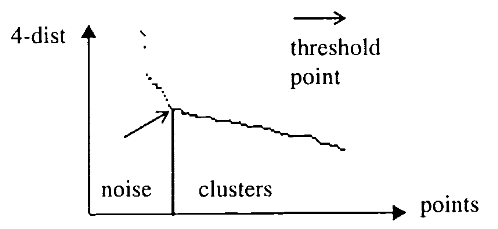
\includegraphics{TheorethicalFramework/K-dist-elbow.png}
    \caption{K-dist plot example for $minPts = 4$ based on a 2-dimensional dataset \citep{ester_density-based_nodate}}
    \label{k-dist-plot}
  \end{figure}

  %The epsilon value is crucial for the DBSCAN algorithm and highly dependent on the dataset \todo{Source}.
  Since we employ various types of datasets and algorithms, it is desirable to have an automated method for determining the epsilon (radius) value.
  The epsilon could influence the results as the radius determines the clusters.
  For this reason, research has also been conducted on an extension of DBSCAN called OPTICS.}

%In conclusion, K-Means and \gls{ap} have straightforward methods for determining hyperparameters.
%For K-Means, the elbow method is the most common, and for \gls{ap}, the median is used for the preference.
\gls{dbscan} is a little more complicated due to the variety of datasets and noise-altering mechanisms we experiment with.
This complexity is why we use \gls{optics} to determine the best value for $radius(\epsilon)$ and choose $minPts$ based on the number of features times two.

\mycomment{\subsection{Overfitting}
  Overfitting is dangerous for machine learning models and one of the biggest mistakes with training machine learning models \citep{demsar_hands-training_2021}.
  It occurs when a machine learning model is trained on samples that are not representative of future test data \citep{bashir_information-theoretic_2020}.
  A common mistake is to evaluate a model using the same data as it is trained on \citep{demsar_hands-training_2021}.
  The model appears to have high accuracy but just memorized the properties of a training dataset.
  Another cause of overfitting can be the size of the training data \citep{valdenegro-toro_machine_2022}.

  To measure if a model overfits, it is necessary to compute the generalization gap \citep{valdenegro-toro_machine_2022}.
  \begin{equation}
    L_{gap} = L_{val} - L_{train}
  \end{equation}
  Where $L{val}$ and $L_{train}$ are the validation and training splits of the dataset.
  For splitting a dataset, a common approach is to have 50\% training data, 30\% for validation and 20\% test \citep{chicco_ten_2017}.
  In addition to this, if a dataset is too small cross-validation can be considered.

  \todo[inline]{Needs more work for unsupervised / cluster problems}

  In summary:
  \begin{enumerate}
    \item It is necessary to evaluate a machine learning model on a dataset that was not used to train the model.
    \item Use a representative training dataset, to work well on unseen data.
    \item To reduce the chance of overfitting for supervised learning, it is a good practice to validate using a 30\% subset.
  \end{enumerate}
}

\subsection{Evaluation methods} \label{theory:evaluate}
Clustering comparison measures are important in cluster analysis for external validation by comparing clustering solutions to a "ground truth" clustering \citep{vinh_information_nodate}.
These external validity indices are a common way to assess the quality of unsupervised machine learning methods like clustering \citep{warrens_understanding_2022}.
A method that could be used for this is the Rand Index \citep{rand_objective_1971}.
It is a commonly applied method for comparing two cluster algorithms \citep{wagner_comparing_nodate}.
An improvement of this method is adjusted for chance by considering the similarity of pairwise cluster comparisons \citep{vinh_information_nodate}.
Both the Rand Index (RI) and Adjusted Rand Index (ARI) \citep{hubert_comparing_1985} report a value between 0 and 1.
Where 0 is for no-similarity and 1 for identical clusters.
Alternatives for RI are the Fowles-Mallows Index and Mirkin Metric.
However, these two methods have their disadvantages. They are, respectively, sensitive to a few clusters and cluster sizes \citep{wagner_comparing_nodate}.
The ARI metric suffers from cluster size imbalance as well, so it only provides not a lot of information on smaller clusters \citep{warrens_understanding_2022}.
Instead, they recommend using the cluster index metric proposed by Fränti et al. \citep{franti_centroid_2014}.

Another popular group of methods is the information theoric-based measures \citep{vinh_information_nodate}.
This metric measures the information between centroids; the higher the value, the better \citep{vinh_information_nodate}.
\gls{mi} is a metric that calculates the probability of an element belonging to cluster $C$ or $C`$.
But, it is not easy to interpret as it does not have a maximum value \citep{wagner_comparing_nodate}.
To this end, \gls{nmi} can be used to report a value between 0 and 1 using the geometric mean \citep{strehl_cluster_2002}.
The metric also exists in an adjusted version as \gls{ami}.
This metric works in the same way as for the \gls{ari} and is mainly needed if the number of data items is small in comparison to the number of clusters \citep{vinh_information_nodate}. \newline

Besides the external validity measurements for clustering, it is also possible to use internal validation methods.
These metrics focus entirely on the intrinsic dataset properties instead of relying on an external baseline cluster algorithm \citep{craenendonck_using_nodate}.
They are assessing two essential concepts of clustering: compactness and separation \citep{hassani_using_2017}.
Both studies consider three different metrics and measure both concepts at the same time \citep{hassani_using_2017}:
\begin{enumerate}
  \item \gls{chi} \citep{calinski_dendrite_1974} is used to measure the cluster variance (well-separated clusters) and low variance within the clusters (tightly coupled data). A high score indicates better clustering.
  \item Silhouette Index \citep{rousseeuw_silhouettes_1987} This metric is similar in measuring cohesion within and separating clusters.
        However, this metric uses the pairwise distance \cite{hassani_using_2017}.
        A score of -1 indicates incorrect clustering and +1 for dense clusters \cite{rousseeuw_silhouettes_1987}.
  \item Davies-Bouldin \citep{davies_cluster_1979} uses the average distance between centroids. A lower score indicates good clustering.
\end{enumerate}

K-Means scores relatively high for \gls{chi} \citep{craenendonck_using_nodate,hassani_using_2017} and SI \citep{craenendonck_using_nodate}.
The same applies to DBSCAN, which scores relatively high on SI and DB due to noise sensitivity \citep{craenendonck_using_nodate}.

% Thus, these metrics are difficult to use for very different cluster algorithms \cite{craenendonck_using_nodate}.
\subsubsection{Existing literature}
%A recent and much-cited study uses \gls{ari} and accuracy as metrics for evaluating K-Means \cite{ahmed_k-means_2020}.
%The accuracy is measured by calculating the percentage of the correct predicted labels and their truth labels.
Comparable studies with differential privacy use external validation \citep{xia_distributed_2020, sun_privbv_2022}.
Their experiment setup uses a so-called non-private cluster algorithm as external validation.
This cluster algorithm is trained without the perturbed data and compared with the same clustering algorithm trained with perturbed data.
Thus, the non-private variant provides the ground truth as an external validation.

They compare the mutual information between a baseline cluster algorithm using \gls{ami} \citep{9679364} or \gls{nmi} \citep{xia_distributed_2020,sun_privbv_2022}.
Another study for evaluating \gls{dp} with \gls{ap} uses both \gls{ari} and \gls{ami}.
In addition to mutual information and rand index scores, it is also not uncommon to calculate the error between the two cluster algorithm's centroids \citep{xia_distributed_2020, 9679364}.
These two studies used Relative Error (RE) for this.

\subsubsection{Research direction}
This chapter outlines the evaluation methods used and provides a definition and brief explanation for each method.

In the literature, both internal and external evaluation methods are commonly used.
While some studies choose one over the other, this thesis will perform both validations.
This approach is crucial to measure how well the data shape is preserved (internal validation) and how the algorithm performs in real-world scenarios (external validation).

Since certain cluster algorithms may score higher or lower on specific metrics, it is essential to choose two metrics for each type of validation.
Based on existing studies and the literature, we have selected metrics adjusted to compensate for the data distribution characteristics.
Hence, we will focus on these metrics' "adjusted" variants:
\begin{enumerate}
  \item Internal validation:
        \begin{enumerate}
          \item \textbf{Calinski Harabasz Index:}
                The definition of \gls{chi} is defined in several steps \citep{liu_understanding_2010}:
                The first definition is the between cluster sum of squares.
                \begin{equation}
                  B = \sum_{i=1} n_i \cdot (C_k - C)^2
                \end{equation}
                \begin{enumerate}
                  \item $n_k$ is the number of data points in cluster $k$.
                  \item $C_k$ is the centroid of cluster $k$.
                  \item $C$ is the dataset centroid
                \end{enumerate}
                The second part of the definition is defined as follows:
                \begin{equation}
                  W_k = \sum_{i=1}n_i \cdot (x_i - C_k)^2
                \end{equation}
                $W_k$ is the within-cluster sum of squares and $x_i$ is the $i$th data point.
                Finally, the \gls{chi} is calculated by combining the between and within-cluster calculations:
                \begin{equation}
                  CH = \frac{B}{\sum_{k=1}^{K}} \cdot \frac{N - k}{k - 1}
                \end{equation}
                \begin{enumerate}
                  \item $K$ is the number of clusters.
                  \item $N$ is the number of data points.
                \end{enumerate}

          \item \textbf{Silhouette coefficient:} This metric is defined as follows \citep{liu_understanding_2010,rousseeuw_silhouettes_1987}:
                \begin{equation}
                  s(i) = \frac{b(i) - a(i)}{max(b(i) - a(i))}
                \end{equation}
                \begin{enumerate}
                  \item $s(i)$ is the silhouette coefficient for a single datapoint $i$.
                  \item $a(i)$ is the mean distance of $i$ and all the other points in the same cluster.
                  \item $b(i)$ is the mean distance of $i$ and all the other points in the next nearest cluster.
                \end{enumerate}
                Finally, the final silhouette score is the mean of all datapoint coefficients $s(i)$.
        \end{enumerate}
  \item External validation:
        \begin{enumerate}
          \item \textbf{Adjusted Rand Index:}
                The \gls{ari} is defined in two steps, one to calculate the actual Rand Index and the other to adjust it for chance.
                The Rand Index formula is defined as follows \citep{hubert_comparing_1985}\footnote{Explaination is part of Sklearn: \url{https://scikit-learn.org/stable/modules/clustering.html}}:
                \begin{equation}
                  RI = \frac{a + b}{C_2^N}
                \end{equation}
                \begin{enumerate}
                  \item $C$ the ground truth elements (So the actual correct predictions/ classes).
                  \item $a$ is the number of pairs of elements part of the ground truth $C$ and part of the predicted class.
                  \item $b$ is the number of pairs of elements in different sets of $C$ and different sets of the predicted class.
                  \item $C_2^N$ is the total number of pairs of elements in the dataset.
                \end{enumerate}
                To compensate for the amount of clusters, the adjusted formula is defined as follows \citep{sinnott_chapter_2016}:
                \begin{equation}
                  ARI = \frac{RI - Expected(RI)}{max(RI) - Expected(RI)}
                \end{equation}
          \item \textbf{Adjusted Mutual Information:}
                As was the case for the \gls{ari}, the \gls{ami} is also defined in two steps.
                The first step is to calculate the actual \gls{mi}, and the second is to adjust it for chance.
                The \gls{mi} is defined as follows \citep{vinh_information_nodate}:
                \begin{equation}
                  H = - \sum_{i=1}^{U} p(i) \cdot log p(i)
                \end{equation}
                $H$ is the uncertainty for one variable given another variable.
                So it can be used to measure the (dis)similarity between two variables.
                \begin{enumerate}
                  \item $U$ is a label to calculate the uncertainty for.
                  \item $p(i)$ is the probability of a random point $i$ falling into class/labe $U$.
                \end{enumerate}
                This same calculation is executed for the second label $V$ and divided by each other.
                \begin{equation}
                  MI = \frac{MI - Expected(MI)}{mean(H(U), H(V)) - Expected(MI)}
                \end{equation}
        \end{enumerate}
\end{enumerate}
%\textbf{Calinski Harabasz Index:} \newline
%\textbf{Silhouette coefficient:} \newline
%\textbf{Adjusted Rand Index:} \newline
%\textbf{Adjusted Mutual Information:} \newline
